\chapter{Model}
\subsubsection*{Mikhail Poberezhnyi(s0558681), Konstantin Kochetov(s559121), Sergey Wolf(s0553749)}
\label{cha:model}

In order to define a property graph model, we have to take into account several constraints:

\begin{itemize}
\item[-] Neo4j supports only directed relationships. It is possible to perform search queries regardless of the direction of the graph, but the direction has to be present when creating a relationship;
\item[-] There is no possibility in Neo4j to save objects (or maps, dictionaries) as properties of nodes or relationships. Property can only be a key-value pair or a key with a list of values;
\item[-] We have to think in terms of queries that are necessary to answer our hypotheses;
\item[-] We can take advantage of the Neo4j APOC library to construct virtual relationships for our analysis without changing the property graph model itself and without creating redundant relationships.
\end{itemize}

\begin{figure}[h]
 \centering
 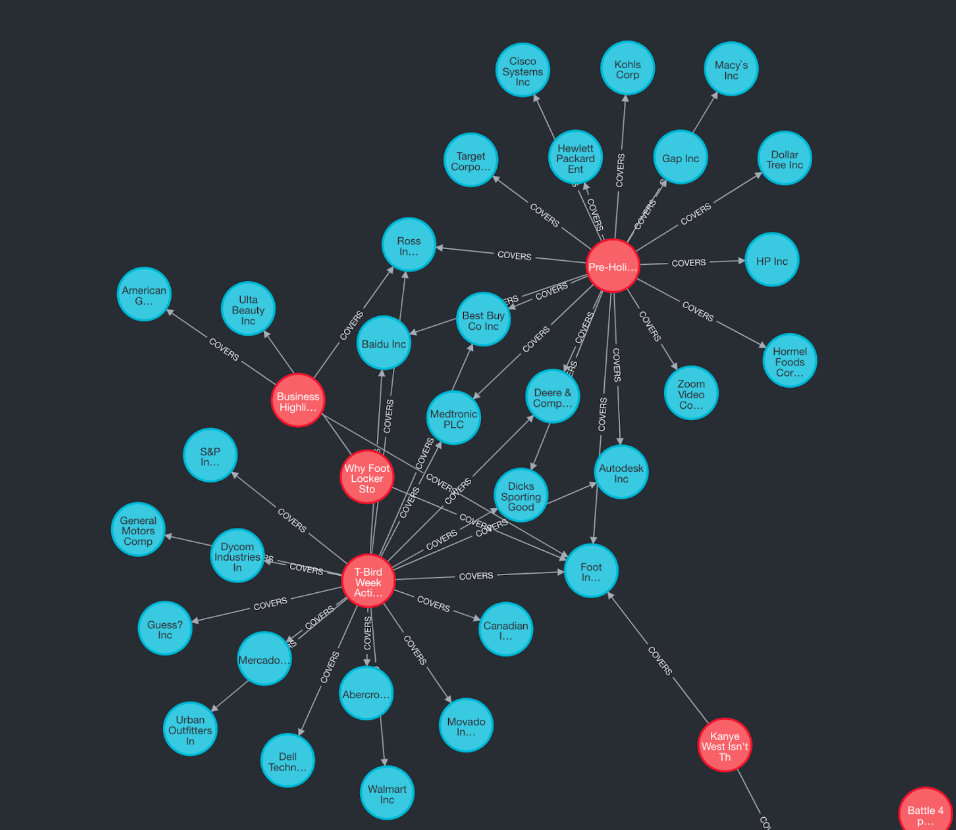
\includegraphics[width=0.8\textwidth]{images/virtual-relationship-between-nodes.png}
 \caption{Relationships between news and companies }
 \label{fig:virtual-relationship-nodes}
\end{figure}


\noindent In tables \ref{table:graph-model-properties} and \ref{table:model-properties-relationships} we see our property graph model and the relationships within:

\begin{table}[h]
\centering{
\begin{tabular}{|l|l|l|}
\hline
\textbf{Node}     & \textbf{Relationship} & \textbf{Node}            \\ \hline
NewsItem & COVERS       & Company         \\ \hline
NewsItem & HAS          & TickerSentiment \\ \hline
NewsItem & HAS          & Topic           \\ \hline
Company  & IS\_IN       & Sector          \\ \hline
Company  & HAS          & Price           \\ \hline
\end{tabular}%
}
\caption{Graph model properties }
\label{table:graph-model-properties}
\end{table}

\begin{table}[h]
\centering{
\begin{tabular}{|l|l|l|}
\hline
\textbf{Node/Relationship}     & \textbf{Properties}\\ \hline
NewsItem & \begin{tabular}[c]{@{}l@{}} - url \\ - time\_pusblished \\ - summary \\ - overall\_sentiment\_score \\ - overall\_sentiment\_label
\end{tabular} \\ \hline
Company & \begin{tabular}[c]{@{}l@{}} - ticker \\ - name \\ - description \\ - company\_sector\_name \\ 
\end{tabular} \\ \hline
Topic & \begin{tabular}[c]{@{}l@{}} - topic \\ - relevance\_score \end{tabular} \\ \hline
Sector  & \begin{tabular}[c]{@{}l@{}} - sector\_name  
\end{tabular} \\ \hline
Price  & \begin{tabular}[c]{@{}l@{}} - company\_ticker \\ - date \\ - open \\ - close \\ 
\end{tabular} \\ \hline
\end{tabular}%
}
\caption{Model properties relationships }
\label{table:model-properties-relationships}
\end{table}

\noindent Overall, such a property graph model, saved in Neo4j, allows us to perform necessary queries to analyse the news coverage of the stock market.

\noindent Figure \ref{fig:virtual-relationship-nodes} shows the visualisation of the relationship between nodes NewsItem (red colour) and Company (blue colour).\\
\\
\noindent Figure \ref{fig:virtual-relationship-nodes-sectors} shows the visualisation of the virtual relationship between nodes NewsItem (red colour) and Sector (orange colour). \\
\\
While NewsItem does not have a direct relationship to Sector, we can create a virtual one (called ``COVERS\_INDUSTRY``) while performing a search query. It is done without changing our underlying graph model. 
\\
That is possible because NewsItem has a direct relationship to Company, and Company has a direct relationship to Sector.

\begin{figure}[h]
 \centering
 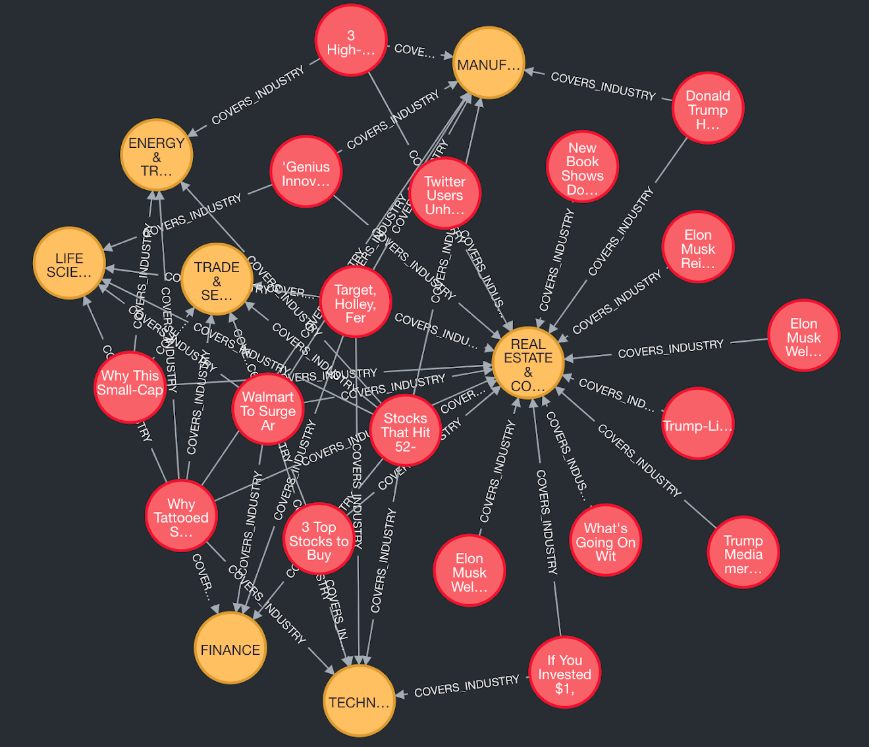
\includegraphics[width=0.8\textwidth]{images/virtual-relationship-between-nodes-sectors.png}
 \caption{Virtual relationship between news and sectors }
 \label{fig:virtual-relationship-nodes-sectors}
\end{figure}

\newpage

\noindent To create such a model from the data we gathered, we had to write several algorithms, as well as our own database parser. Here is a short explanation of the implementation part:

\begin{itemize}
\item[-] we perform breadth-first-search, where the first node is a randomly selected company;
\item[-] we request the news for a certain range for this company (one month); 
\item[-] if the news article was visited before, we ignore it;
\item[-] we save news article, its topic, sentiment for every company mentioned, as well as each company itself, in the database;
\item[-] We gather the following information for every company mentioned: what industry sector the company is, as well as one month of stock price data in the month the news article was published;
\item[-] if the company is encountered again, we request the news starting from the previous earliest date
\end{itemize}